%!TEX root = ../dissertation.tex
\begin{savequote}[75mm]
Nulla facilisi. In vel sem. Morbi id urna in diam dignissim feugiat. Proin molestie tortor eu velit. Aliquam erat volutpat. Nullam ultrices, diam tempus vulputate egestas, eros pede varius leo.
\qauthor{Quoteauthor Lastname}
\end{savequote}

\chapter{A11Y Tool}
With the successful completion of the A11Y Guide sufficient knowledge had
been gained within the accessibility domain to enable the production of a
tool to identify issues. The fundamental idea behind the tool is to reduce
the feedback loop (and thus the price) of discovering accessibility issues. To
keep the project to a sensible scope the tool will form the "means" by which
accessibility testing could be undertaken but will be limited in the number
of accessibility issues it will identify.

\section{Preparation}
\subsection{Current Process}
The current projects

\subsection{Understanding current solutions}
Prior to building my own I wanted to survey the current landscape of
accessiblity tools. Thanks to the A11Y Guide I had already collected a list of
current testing tools. All but one of the tools target the browser through a
bookmarklet.

\begin{table}[h!]
\centering
\begin{tabular}{ |c|c|c|c| }
 \hline
 Tool & Method & Good & Bad  \\
 \hline
 \hline
 Axe Core & Bookmarklet/Extension &  & a \\
 \hline
 HTML Code Sniffer & Bookmarklet & b & b \\
 \hline
 ESLint JSX A11Y & IDE/CLI & c & c \\
 \hline
 Tota11y & Bookmarklet & d & d \\
 \hline
\end{tabular}
\end{table}

\subsection{What makes this tool different?}


\subsubsection{Browser vs IDE}
Two possible methods for identification of issues

The browser was chosen because


\subsection{Generating ideas}

\subsection{Defining Requirements}

\subsection{Design}
Fig.~\ref{fig:tool_current_design} demonstrates the rough design for most of
the current tools. They typically have tightly coupled components for
applying rules and displaying results which limits the way in which the
testing can be done.

\begin{figure}[H]
\centering
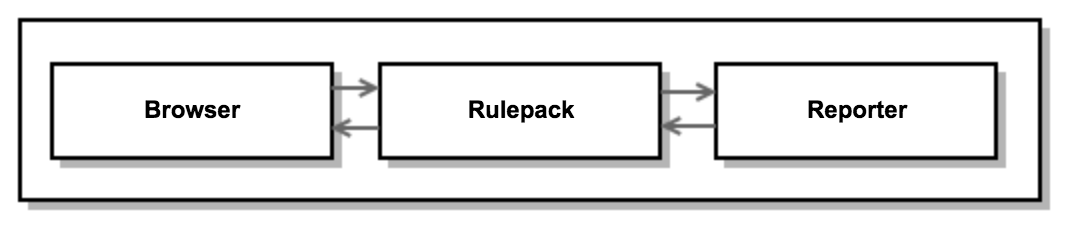
\includegraphics[width=0.8\textwidth]{figures/a11y_tool_current_design}
\captionsetup{justification=centering}
\caption{Current tool design
\label{fig:tool_current_design}}
\end{figure}

% TODO - reference IOC http://www.laputan.org/drc/drc.html
The main limitation in such designs is reusability and customisation. Coming
from a Java background we tend to apply the inversion of control principle to
decouple the reusable components from the specific ones. This comes with the
added benefit of being able to build and test specific modules in isolation.
Fig.~\ref{fig:tool_proposed_design} demonstrates how I propose to apply
this and the next few sections in the report will document each component.

\begin{figure}[H]
\centering
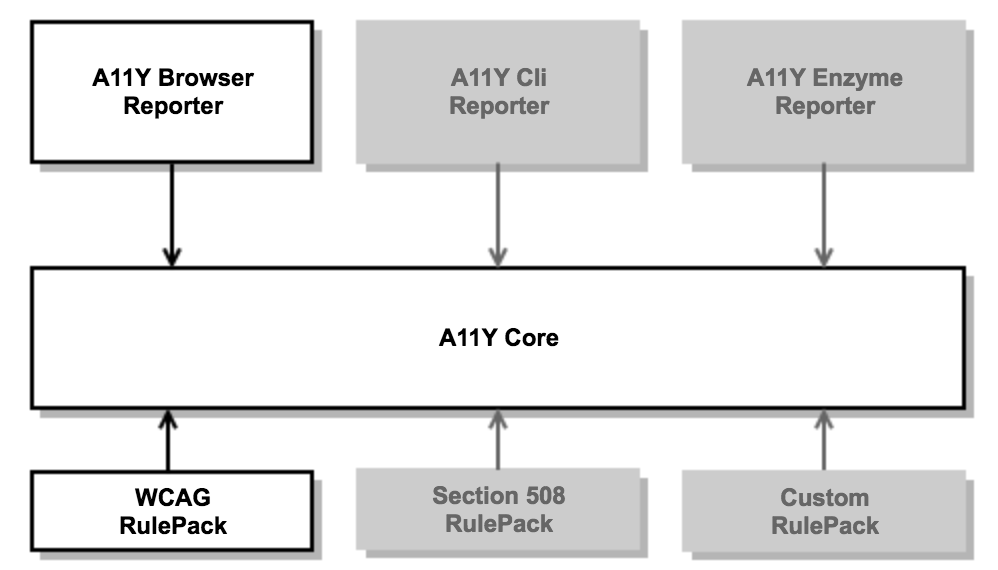
\includegraphics[width=0.5\textwidth]{figures/a11y_tool_proposed_design}
\captionsetup{justification=centering}
\caption{Proposed tool design
\label{fig:tool_proposed_design}}
\end{figure}

\subsubsection{A11Y Core}
This component will form the fundamental pieces of the tool. It will define
interfaces and common implementations. It will be broken down into 'Worker',
'Checker', and 'Result'.

A 'Checker' offers a method to check content for issues and give detail
about what content they are checking. Fig.~\ref{fig:checker_design} demonstrates
how 'Checker' can be extended to implement different checks against a web page.

\begin{figure}[H]
\centering
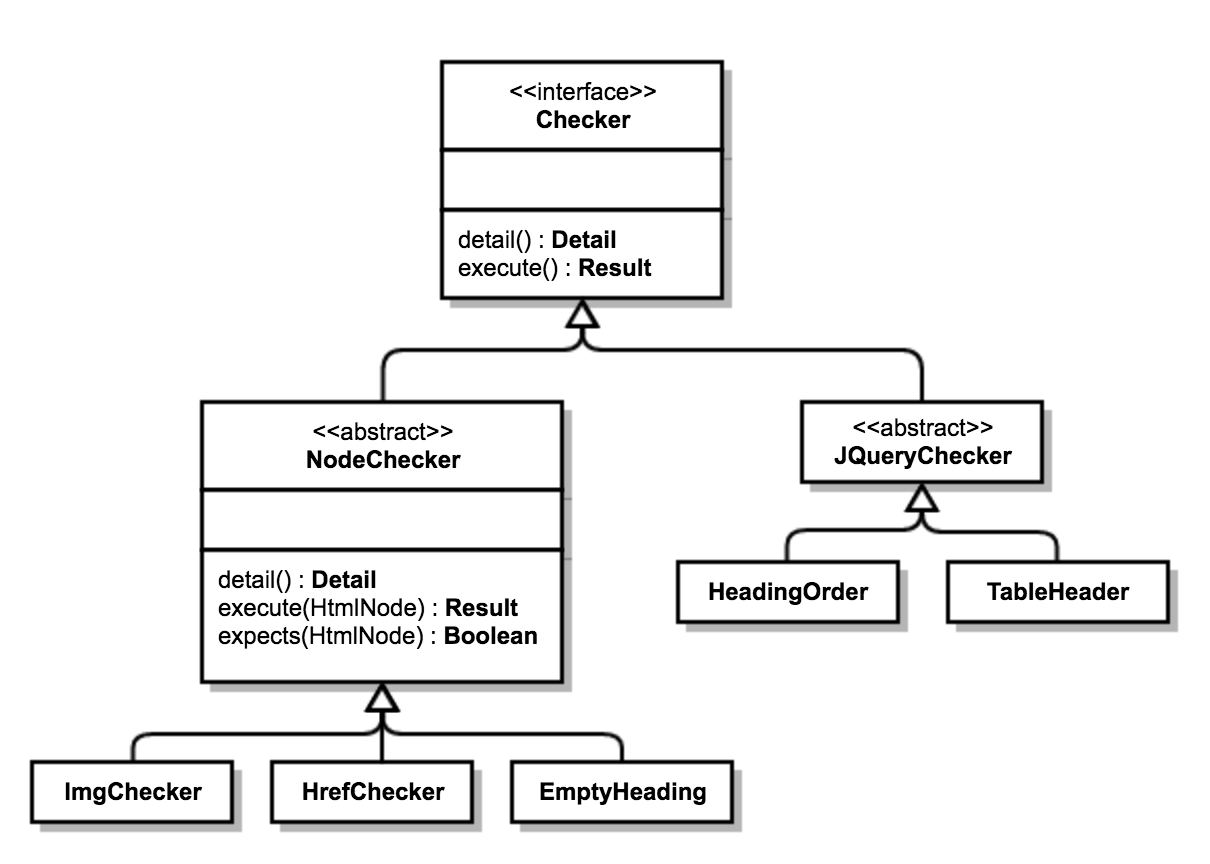
\includegraphics[width=0.6\textwidth]{figures/a11y_tool_checkers}
\captionsetup{justification=centering}
\caption{Proposed 'Checker' inheritance structure
\label{fig:checker_design}}
\end{figure}

A 'Result' is an outcome of a 'Checker' and by default will take the form of
Success, Warn, Info or Error. They hold the test that was executing and
what the test was applied against. Error and Warn have an additional property of
remeidation which is to be defined by the 'Checker' to offer a recommended
method to fix the identified issue. Fig.~\ref{fig:result_design} demonstrates
this structure. It is unlikely that anyone would extend 'Result' but it is
possible if required.

\begin{figure}[H]
\centering
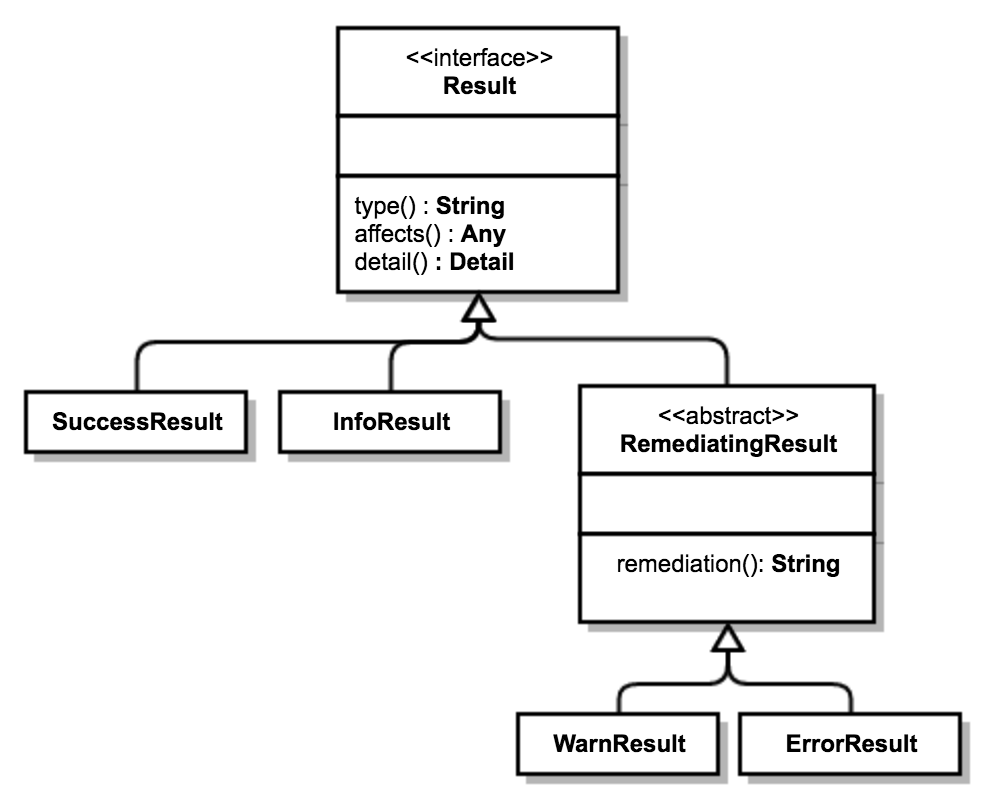
\includegraphics[width=0.6\textwidth]{figures/a11y_tool_result}
\captionsetup{justification=centering}
\caption{Proposed 'Result' inheritance structure
\label{fig:result_design}}
\end{figure}

The concept of a 'Worker' was added late on during the implementation phase as a
direct result of the performance of 'Checker's being poor. Performance issues
were noticeable when iterating around a web pages with a large number of DOM
elements. The worker inverted the for loop and meant that
rather than iterating around the DOM within each 'Checker' The DOM was
iterated around only once and each checker was called to perform it's check
only if that DOM node was relevant to it.

Workers implement the Singleton Pattern as only a single instance of them is
desired.



\subsubsection{User interface}

\section{Deliverable}


\subsection{A11Y Tool Core}
Singleton pattern



\subsection{A11Y Tool Browser}
\newthought{Lorem ipsum dolor sit amet},

This chapter should describe what was actually produced: the programs which
were written, the hardware which was built, the theory which was developed or
the new scientific knowledge acquired.

For software projects, give a high-level overview of your realisation of the
design. Describe the general organisation of any body of code, web pages,
database tables, etc, that you have created. Highlight any particularly
noteworthy aspects, e.g., specialised algorithms, but avoid excessive low-level
detail. Diagrams and examples are usually valuable.

For research projects, provide a detailed overview of how the research was
executed (e.g., participants involved, etc). the research results and their
analysis. Include a description of any statistical analysis methods used.
Highlight any particularly noteworthy aspects, e.g., especially interesting
results. Graphs/charts and examples are usually essential. When reporting
statistical analysis, do not merely present the statistics without interpreting
their meaning for the reader – e.g., what are the implications of the findings?
Where applicable, based on the results and analysis, present a set of
recommendations, guidelines, or itemised list of contributions to knowledge
that may be derived from your work.

This section should be answering the question: “What did the project actually
produce?”
